% chap4.tex
%

\mychapter{Non-factoid Question Answering}
\label{chapter:non-factoid}

\noindent

In this chapter I summarize the proposed work in developing a non-factoid question answering system.
In particular, Section \ref{sec:non-factoid:architecture} described the general architecture of the system, and the following chapters describe the proposed improvements to different stages of the pipeline.

\section{The architecture of the system}
\label{sec:non-factoid:architecture}

\begin{figure}[h]
\centering
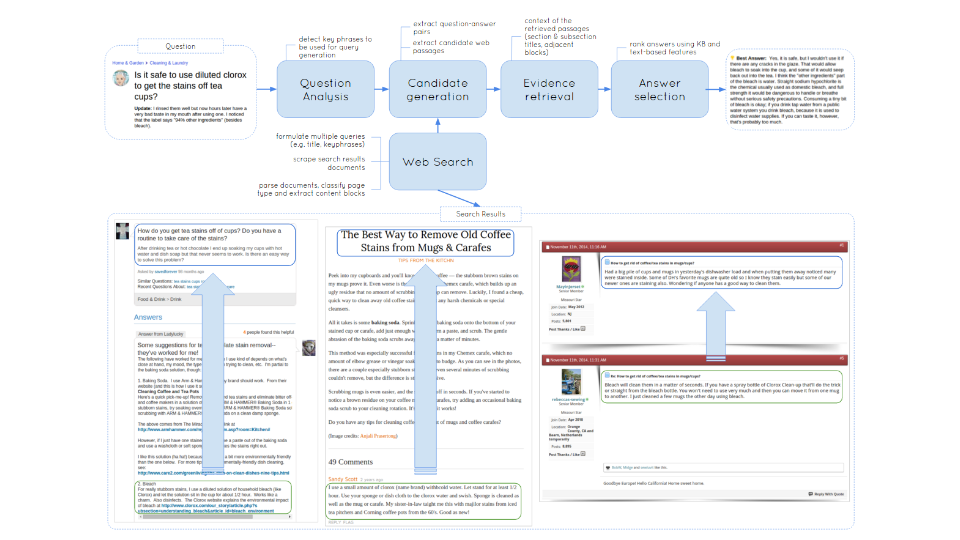
\includegraphics[width=\textwidth]{img/web_page_structure_nonfactoid}
\caption{Using web page structure information for non-factoid question answering}
\label{fig:non-factoid:architecture}
\end{figure}

The architecture of the system I develop is somewhat standard and contains 4 main stages: question analysis, candidate generation, evidence retrieval and answer selection.
Figure \ref{fig:non-factoid:architecture} depicts the question-answering pipeline.

\subsection{Question Analysis}
\label{sec:non-factoid:architecture:analysis}

Questions that users post to CQA websites often contain title and body and can be relatively long and contain multiple important and not so important context information and details.
The success of the retrieval-based question answering system depends on the information it finds in a collection.
Extra long search queries are not very efficient and can return few or zero results.
Therefore, there is a problem of summarizing the user question.
Some strategies often used include considering first part of the question, \eg title of the question only.
However, often the most important part of the question isn't the title, or the title doesn't contain all the crucial information, \eg\\
\textbf{Title}: \textit{Diet please please help asap?}\\
\textbf{Body}: \textit{I want to lose weight, at least 4 stone but I don't know what I should eat :( what should I have for breakfast lunch and dinner? Should I exercise a little? Please help!!}

To summarize the question I propose to use recent advances in the field of deep learning, in particular a model similar to \cite{rush-chopra-weston:2015:EMNLP}.
In more detail, I propose to train neural network based summarization model to generate the summary of the question, which will be used as a query to retrieve similar questions.
Such a model can be specifically trained to maximize retrieval performance on a collection of question-answer pairs, retrieved by systems in LiveQA TREC 2015 and labeled by NIST assessors.

\subsection{Structure of the Web Page for Candidate Generation and Scoring}
\label{sec:non-factoid:architecture:page-structure}

The diversity and complexity of non-factoid questions pose additional challenges for automatic question answering systems.
To answer such questions a system often needs to provide a whole paragraph of text, \eg TREC LiveQA'15 limits the answers to a maximum of 1000 characters.
Therefore, a candidate answer becomes much longer, which requires additional attention on candidate generation and ranking stages.

% Is this related work? Or here?
Existing techniques usually extract one or more consecutive sentences not exceeding the maximum answer length, pool them together and rank using certain feature representation, by large ignoring the context information from the page where the answer was extracted from.
In the system I develop I propose to utilize the structure of the web page for both candidate generation and scoring.

To generate better candidates I'm going to utilize the structure of retrieved web pages.
The previous analysis showed \cite{savenkov_liveqa15}, that many search results retrieved for the question are FAQs, forums or other community question answering websites.
From such resources it's beneficial to extract question answer pairs, which can be done either be designing wrapper for popular websites, utilizing semantic annotations, such as \hyperref[https://schema.org]{https://schema.org} or by applying some of the automatic question-answer extraction methods \cite{cong2008finding}.
For other resources, page segmentation techniques, similar to \cite{cai2003vips}, can split a page into semantically information blocks, which will help to make sure that candidate don't contain disjoint and unreadable information.

After a candidate passage is extracted, we need to score it as a potential answer.
Often, a passage taken out of context is hard to understand even for human.
Therefore, I propose to include the context information, \ie some features, representing the web page where the passage was taken from and its location there (\eg adjacent passages, which are often related \cite{yang2016beyond}).

\subsection{Answer Summarization}
\label{sec:non-factoid:architecture:summarization}

Unlike factoid questions, where evidence from all retrieved passages is usually aggregates, a traditional non-factoid question-answering system simply returns the top scoring passage as the answer.
However, such an answer can contain a lot of redundant or irrelevant information, whereas other good candidate passages may contain supplemental information or different opinion.
Therefore, an idea to summarize passages and generate the final answer sounds natural in this scenario.
The winning approach from TREC LiveQA'15 included a combination strategy, that simply put together multiple top scoring passages while the answer doesn't exceed the maximum length \cite{diwang_liveqa15}.
In my thesis I'm planning to explore the answer summarization problem in more detail.
More specifically, I propose to explore deep learning techniques, that lie in the core of recent successes in text generation, \eg image caption generation and machine translation models \cite{bahdanau2014neural,xu2015show}.
Answer summarization problem can be posed as answer generation problem using recurrent neural network, that has information about the question and retrieved passages, and it can be trained using existing CQA question-answer pairs and retrieved passages, that can be assumed as the source of the answers.
Alternative and simpler approach is to solve this problem as sequential answer selection problem, where a model is trained to predict the next sentence in the answer.
Such a model can be trained on a collection of questions and answer sentences, which will provide the model information on both answer discourse coherence and relevance.

\section{Evaluation}
\label{sec:non-factoid:architecture:evaluation}

Evaluation of complete non-factoid question answering systems is complicated due to the variability of answer language, the quality of which is impossible to estimate using manually created answer patterns (as is the case for factoid TREC QA dataset).
A manual judgment of answers is needed, and luckily TREC LiveQA 2016 is offering such an opportunity.
The model I'm developing will participate in the shared task, which will allow us to evaluate it against other competing approaches.

The analysis of individual components can be performed using labeled data from TREC LiveQA 2015, which includes passages extracted from Yahoo! Answers as well as regular web documents.
In more detail, the performance of the answer summarization module will be estimated by similar questions retrieval performance, \eg Precision @ N since we are interested in retrieving more relevant answers in TopN rather than good ranking within the retrieved group.
To make results reproducible a collection of Yahoo! Answers QnA pairs from the WebScope\footnote{http://webscope.sandbox.yahoo.com/catalog.php?datatype=l} and Lucene IR library will be used for question retrieval.

The dataset to evaluate the effectiveness of using web page structure for answer scoring will be derived from TREC LiveQA 2015 labels, which include a big number of passages, that were generated from regular web pages.
Therefore, the problem of evaluation of answer scoring methods can be posed as passage ranking problem and metrics, such as Precision@1, can be used as a quality measure.

Finally, the answer summarization module is the most difficult to evaluate, because it's result is a free form text, the quality of which needs to be manually labeled.
Therefore, for this task I will refer to the wisdom of a crowd and use Amazon Mechanical Turk to label the quality of answers and compare to the top scoring passages for the same question.

\section{Summary}
\label{sec:non-factoid:summary}

The proposed research directions target various aspects of non-factoid question answering pipeline and can help improve both precision and recall of existing systems.
The results of this work can help to move in the direction of systems, that produce a natural language response by analyzing the information available on the web.
In the next chapter, I will describe the proposed work and results on interactions between a question answering system and users.

%THIS IS OLD...
%My proposal for non-factoid question answering can be summarized as follows:
%\begin{itemize}
%\setlength\itemsep{0em}
%\item \textbf{CQA candidate generation}: retrieve a set of question-answer pairs by searching a CQA archive\footnote{https://answers.yahoo.com/}
%\item \textbf{Web document retrieval}: retrieve a set of documents by querying web search with the question (and queries generated from it)
%\item \textbf{Web candidate answer generation}: classify web page into one of the following types: article, forum thread, FAQ page, CQA page, other. Extract key elements using type-specific extractors (QnA pairs, FAQ and CQA pages, forum question and posts and article passages with the corresponding titles, subtitles and surrounding text).
%\item \textbf{Ranking}: Rank the generated candidate answers by building on techniques from existing research \cite{surdeanu2011learning}.
%\end{itemize}
